\section{Procedimiento}
Para el presente proyecto, se implement\'o una metodolog\'ia en cascada con las siguientes  actividades:
\begin{figure}[H]
	\caption{Metodolog\'ia de cascada}
	\label{fig:segVideo}
	\centering
	\includegraphics[width=420px,height=80px]{graphics/cascada.PNG} \\
	\textbf{Fuente:} Propia.
\end{figure} 
\subsection{Selecci\'on del movimiento}
El investigador visit\'o a cada equipo deportivo durante los d\'ias de entrenamiento (e.g. Lunes de taekwondo, martes de tenis de mesa y mi\'ercoles de animaci\'on).  Previamente al entrenamiento, el equipo deportivo realizaba series de movimientos que ayudan a calentar y estirar el cuerpo humano.  Luego del calentamiento, el entrenador ense\~naba a los atletas, las t\'ecnicas que ayudan a mejorar el rendimiento deportivo (e.g. Patadas, atrapadas, saques, remates), y posteriormente cada atleta replicaba los movimientos. Por \'ultimo, el investigador con la ayuda del equipo deportivo, seleccionaron un movimiento de calentamiento (e.g. Jumping jacks, patada lateral y saque derecha).
\subsection{Toma de datos}
El investigador visit\'o nuevamente a cada equipo deportivo y esper\'o que finalizara la rutina de calentamiento (durante esa actividad, el investigador instal\'o el prototipo de toma de datos en el lugar asignado), posteriormente al calentamiento, el entrenador seleccionaba a un atleta para participar en la toma de datos (en paralelo, los atletas restantes continuaban con su entrenamiento), el atleta llegaba con el investigador y realizaba dos actividades distintas:
\begin{itemize}
\item La primera actividad constaba en posicionar correctamente al atleta, dicha posici\'on depende de dos condiciones: La primera se chequeaba que se dibuje completamente el seguimiento del esqueleto y la segunda se verificaba que el seguimiento no falle durante la ejecuci\'on del movimiento v\'alido, lo cual se le solicitaba al atleta realizar 2 repeticiones de prueba. S\'i se cumple ambas condiciones, el investigador apuntaba las observaciones de la altura del usuario y la distancia de profundidad entre el sensor y la cadera central del atleta (capturadas por el instrumento de detecci\'on de profundidad).
\item Al encontrar la posici\'on correctamente, el entrenador le programaba al atleta una rutina en base al movimiento seleccionado (la rutina puede ser dos tipos: Por tiempo o por cantidad de repeticiones), posteriormente se terminaba con la grabaci\'on de la rutina del deportista, la cual consist\'ia en grabar repeticiones del movimiento v\'alido.
\end{itemize}
Se debe tomar en cuenta que estas dos actividades se realizaban por cada atleta del equipo deportivo, durante el tiempo de entrenamiento.
 \begin{figure}[H]
	\caption{Fotograf\'ias durante la toma de datos}
	\label{fig:getDataStep}
	\centering
	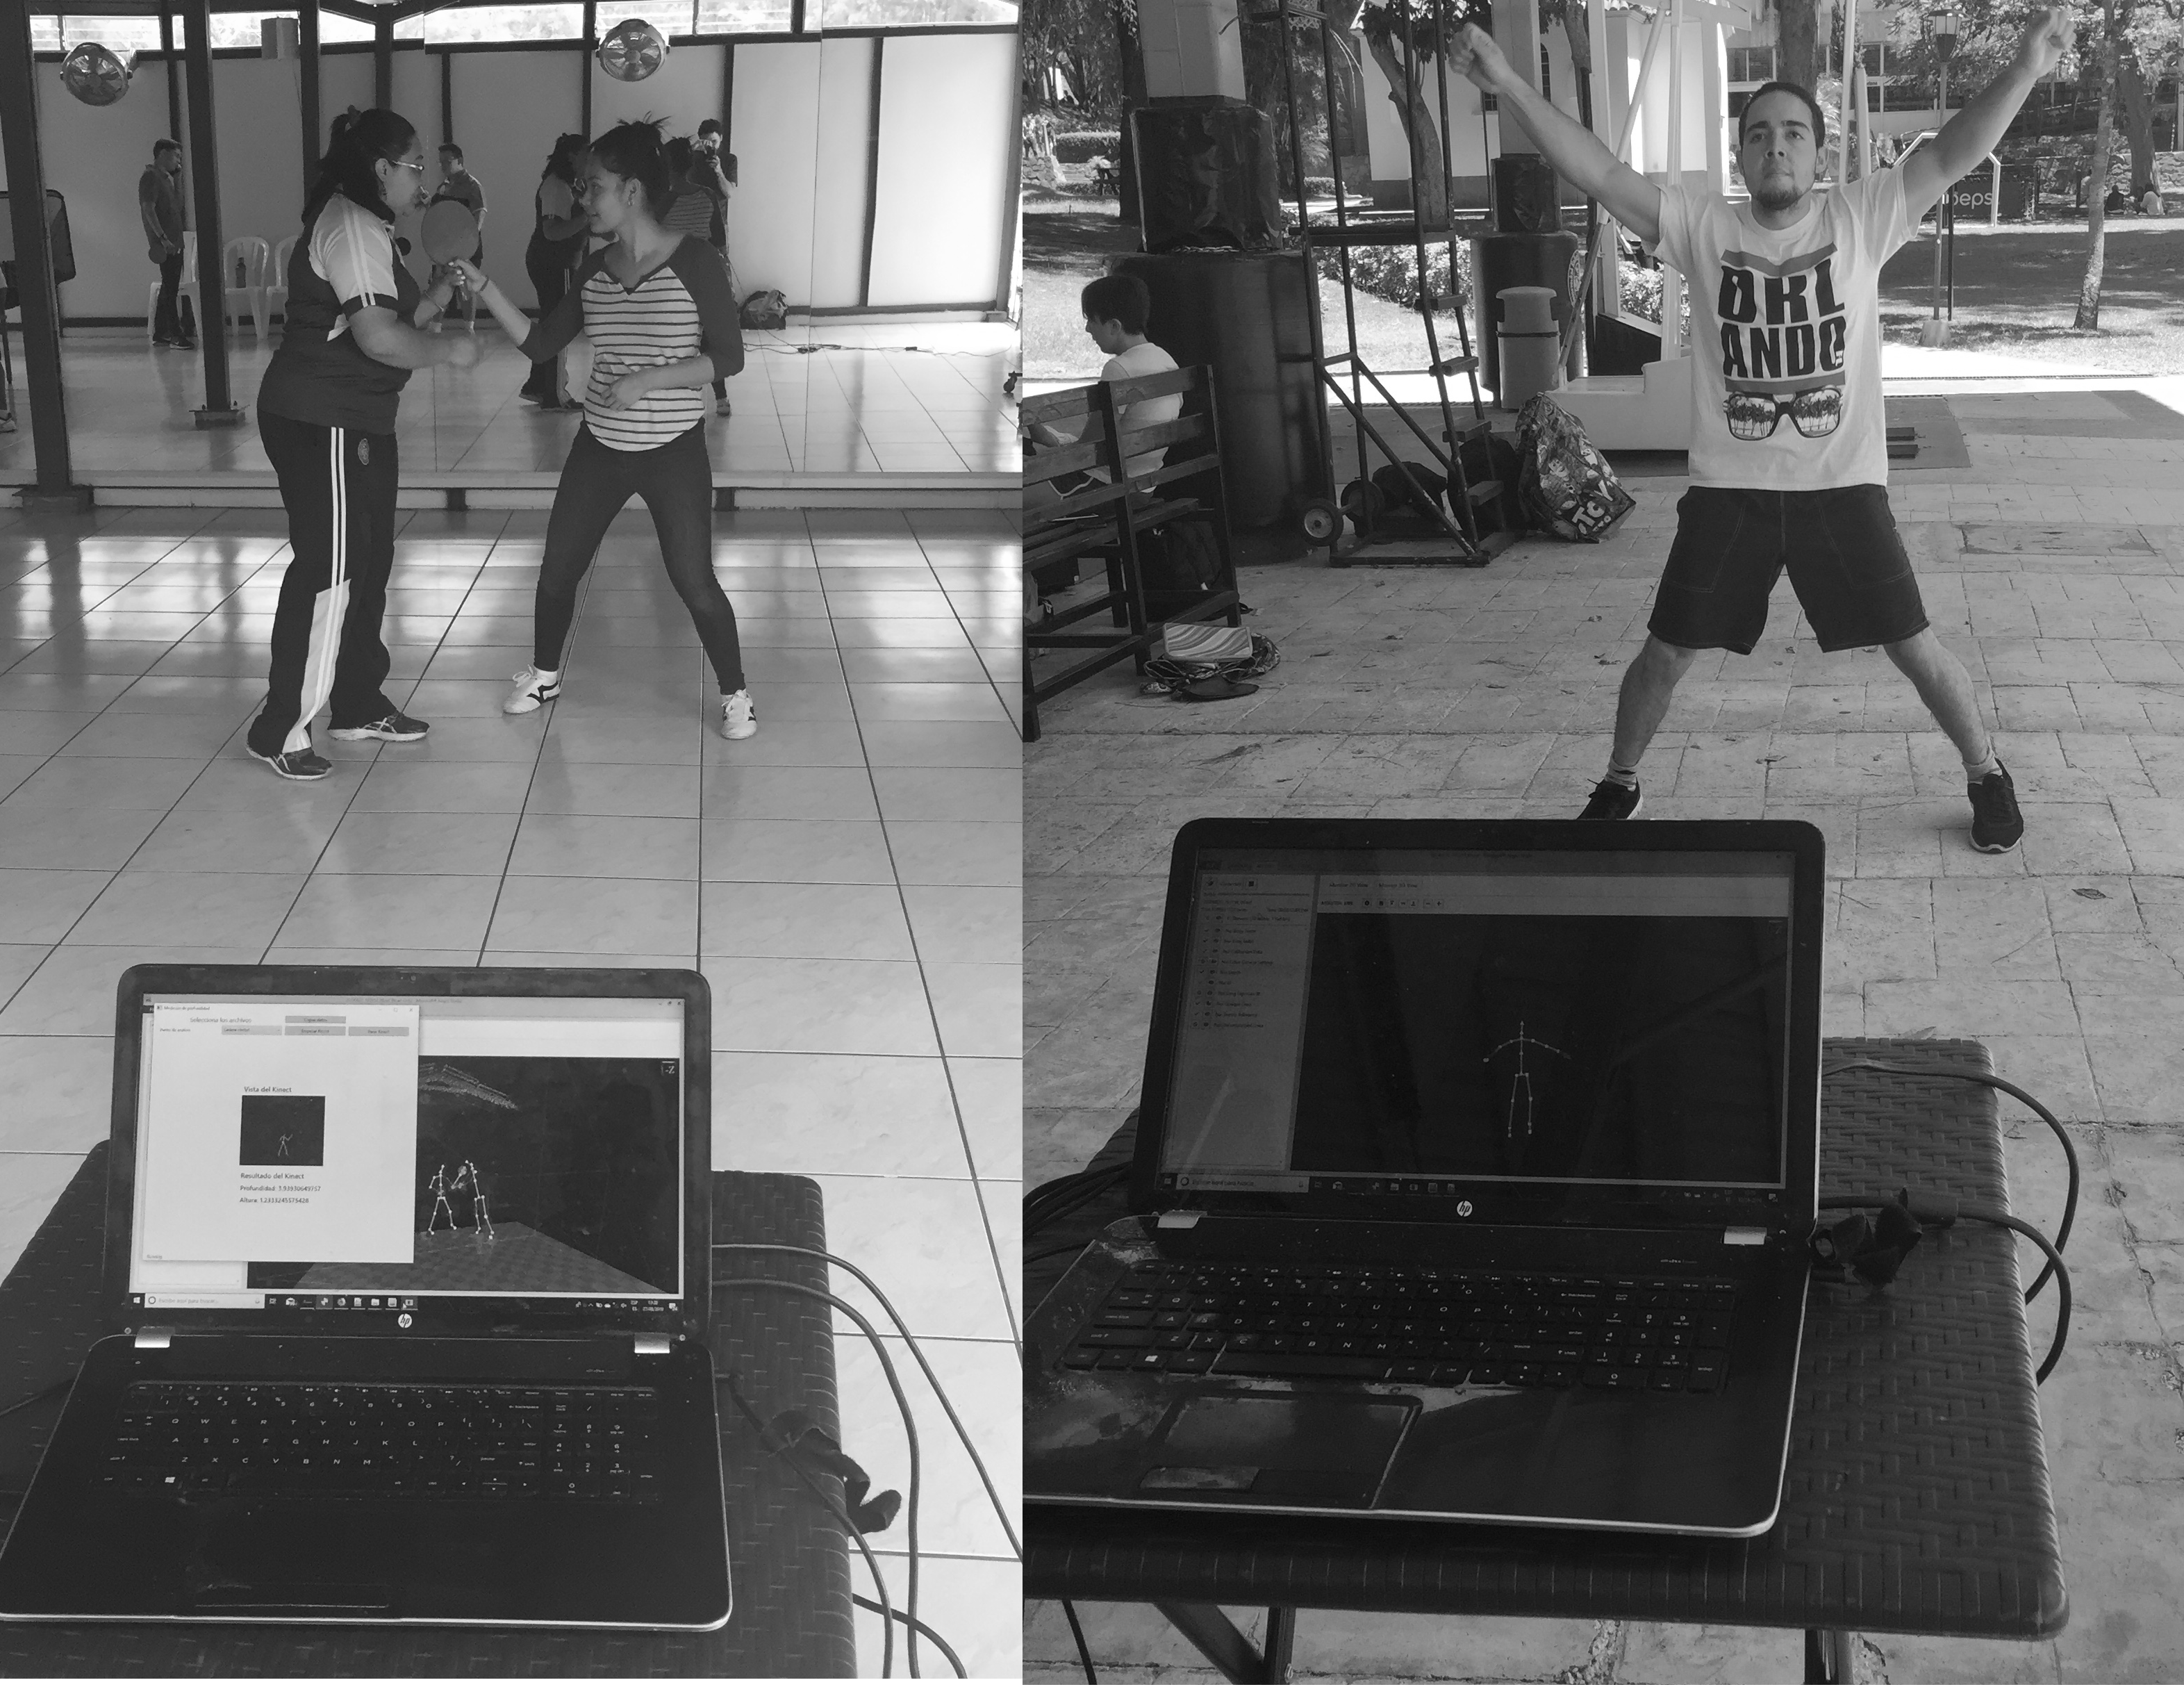
\includegraphics[width=280px,height=280px]{graphics/tomaDatos.png} \\
	\textbf{Fuente:} Propia
\end{figure} 
\subsection{Documentaci\'on del movimiento}
El investigador realiz\'o una breve entrevista a cada entrenador y algunos atletas (similar a un grupo focal), con la finalidad de detallar todos los aspectos de los movimientos, adem\'as de definir los pasos requeridos de cada movimiento v\'alido. Posteriormente a la entrevista, el investigador complet\'o todos los formularios respectivos de movimiento (Formularios de datos de entradas):
\subsubsection{Formularios de entradas de tenis de mesa}
\begin{figure}[H]
	\caption{Formulario de movimiento de tenis de mesa}
	\label{fig:frmMovTen}
	\centering	\includegraphics[width=445px,height=600px]{graphics/resultados/movimientoTenis.PNG} \\
	\textbf{Fuente:} Elaborado por el autor de tesis con base a las observaciones del trabajo de campo
\end{figure}
\begin{figure}[H]
	\caption{Formulario de rutina de tenis de mesa}
	\label{fig:frmRoutTen}
	\centering	\includegraphics[width=445px,height=600px]{graphics/resultados/rutina-tennis.PNG} \\
	\textbf{Fuente:} Propia
\end{figure}
\subsubsection{Formularios de entradas de animaci\'on}
\begin{figure}[H]
	\caption{Formulario de movimiento de animaci\'on}
	\label{fig:frmMovCheer}
	\centering	\includegraphics[width=445px,height=600px]{graphics/resultados/movimientoCheerleader.PNG} \\
	\textbf{Fuente:} Propia
\end{figure}
\begin{figure}[H]
	\caption{Formulario de rutina de animaci\'on}
	\label{fig:frmRoutCher}
	\centering	\includegraphics[width=400px,height=490px]{graphics/resultados/rutina-cheerleaders.PNG} \\
	\textbf{Fuente:} Propia
\end{figure}
\subsubsection{Formularios de entradas de taekwondo}
\begin{figure}[H]
	\caption{Formulario de movimiento taekwondo}
	\label{fig:frmWhiteMov}
	\centering	\includegraphics[width=445px,height=600px]{graphics/resultados/movimientoTaekwondo.PNG} \\
	\textbf{Fuente:} Propia
\end{figure}
\begin{figure}[H]
	\caption{Formulario de rutina de taekwondo}
	\label{fig:frmRoutTaek}
	\centering	\includegraphics[width=445px,height=600px]{graphics/resultados/rutina-taekwondo.PNG} \\
	\textbf{Fuente:} Propia
\end{figure}
\subsection{Etiquetaci\'on de v\'ideos}
El investigador cre\'o desde cero, una base de datos de gesturas por movimiento (a partir del instrumento Visual Gesture Builder), luego se adjunt\'o a la base de datos, todos los v\'ideos recuperados de la actividad de la toma de datos, y por cada v\'ideo se analiz\'o fotograma por fotograma, asignando un valor a cada paso del movimiento, tal como se muestra en la figura de proceso de etiquetaci\'on del movimiento:
 \begin{figure}[H]
	\caption{Proceso de etiquetaci\'on del movimiento derecha}
	\label{fig:getTag}
	\centering
	\includegraphics[width=250px,height=250px]{graphics/etiquetas.png} \\
	\textbf{Fuente:} Propia
\end{figure} 
\subsection{Construcci\'on y pruebas del modelo}
Por cada modelo, el investigador separ\'o los v\'ideos etiquetados en dos partes:
\begin{itemize}
\item \textbf{V\'ideos para el entrenamiento y construcci\'on del modelo:} Elementos que permiten  entrenar el modelo, generando un archivo de base de datos de gesturas (.gdb), la cual proporciona el valor del factor de movimiento a partir del algoritmo Random Forest Regression.
\item \textbf{V\'ideos para an\'alisis:} El investigador seleccion\'o el archivo de bases de datos de gesturas, y posteriormente la herramienta analiz\'o cada v\'ideo, proporcionando el valor real y pronosticado del modelo, tal como se muestra en la figura de obtenci\'on de valores, el valor real es de 0.008018661, mientras que el valor pronosticado es de \num{103893e-6}:
\end{itemize}
 \begin{figure}[H]
	\caption{Obtenci\'on del valor real y pronosticado}
	\label{fig:getError}
	\centering
	\includegraphics[width=300px,height=300px]{graphics/getError.png} \\
	\textbf{Fuente:} Propia
\end{figure} 
\subsection{Selecci\'on y aceptaci\'on del modelo}
\begin{itemize}
\item \textbf{Selecci\'on:} El investigador realiz\'o tres submodelos distintos por movimiento, con distintos datos de entrenamiento (combinaciones de v\'ideos de entrenamientos y an\'alisis). As\'i mismo por cada submodelo se analiz\'o un v\'ideo de an\'alisis, tabulando los datos reales y pronosticado en una hoja de observaciones (Ver anexos, tabla \ref{tab:obsErrores}). Posteriormente al proceso de tabulaci\'on, se calcul\'o los errores correspondientes de cada modelo (error medio pronosticado, desviaci\'on media absoluta y la ra\'iz del error cuadr\'atico medio), seleccionando as\'i el modelo que tenga un menor error. 
\item \textbf{Aceptaci\'on:} El investigador  verifica la media de los errores de cada submodelo, en caso que el error sea mayor o igual  a un medio del valor de reconocimiento (valor recuperado por los formularios del paso de documentaci\'on del movimiento) se rechaza el modelo, en caso contrario, se da la aprobaci\'on y se construye los intervalos de confianza de detecci\'on de los pasos de un movimiento v\'alido, adem\'as de calcular los porcentajes de detecci\'on de movimiento v\'alido e inv\'alido.
\end{itemize}
\subsection{Extracci\'on de datos de los v\'ideos}
Por cada modelo aceptado, el investigador extrajo los datos del tiempo y el recorrido de la mu\~neca derecha de una repetici\'on, con el fin de objetivo de validar que cada modelo fue entrenado con distintos datos, reflejado en una  regresi\'on de tiempo y recorrido. Lo cual para construir dicha regresi\'on, el investigador separ\'o por cada v\'ideo, los renglones de fotogramas de una repetici\'on, listando los tiempos iniciales y finales utilizado para la extracci\'on de datos de v\'ideos .xef (recuperado del instrumento, Kinect studio).
\begin{figure}[H]
	\caption{Segmentos de repeticiones de un v\'ideo}
	\label{fig:segVideo}
	\centering
	\includegraphics[width=420px,height=100px]{graphics/separarPuntos.PNG} \\
	\textbf{Fuente:} Propia
\end{figure} 
\subsection{Validaci\'on  del modelo en tiempo real}
El investigador realiz\'o una \'ultima visita a cada equipo deportivo (cuyo modelo fue aprobado), en dicha visita instal\'o el prototipo del modelo en lugar asignado (en paralelo, los atletas realizaban el calentamiento), posteriormente a la instalaci\'on, el investigador le ense\~n\'o al entrenador una versi\'on de prueba de una rutina tabata, dicha prueba lo realiz\'o el investigador (cabe resaltar que el investigador vest\'ia deportivamente y adem\'as ejecut\'o previamente los ejercicios de calentamiento) con una rutina de 1 serie de 10 segundos de descanso y 50 segundos de trabajo. Luego de la prueba, el entrenador seleccion\'o a un grupo de atletas que no participaron en el proceso de toma de datos, y posteriormente se le program\'o a cada atleta del grupo, una rutina tabata (cada deportista se posicion\'o en la distancia de profundidad recomendada).
 \begin{figure}[H]
	\caption{Fotograf\'ias durante la validaci\'on del modelo}
	\label{fig:getvalidationStep}
	\centering
	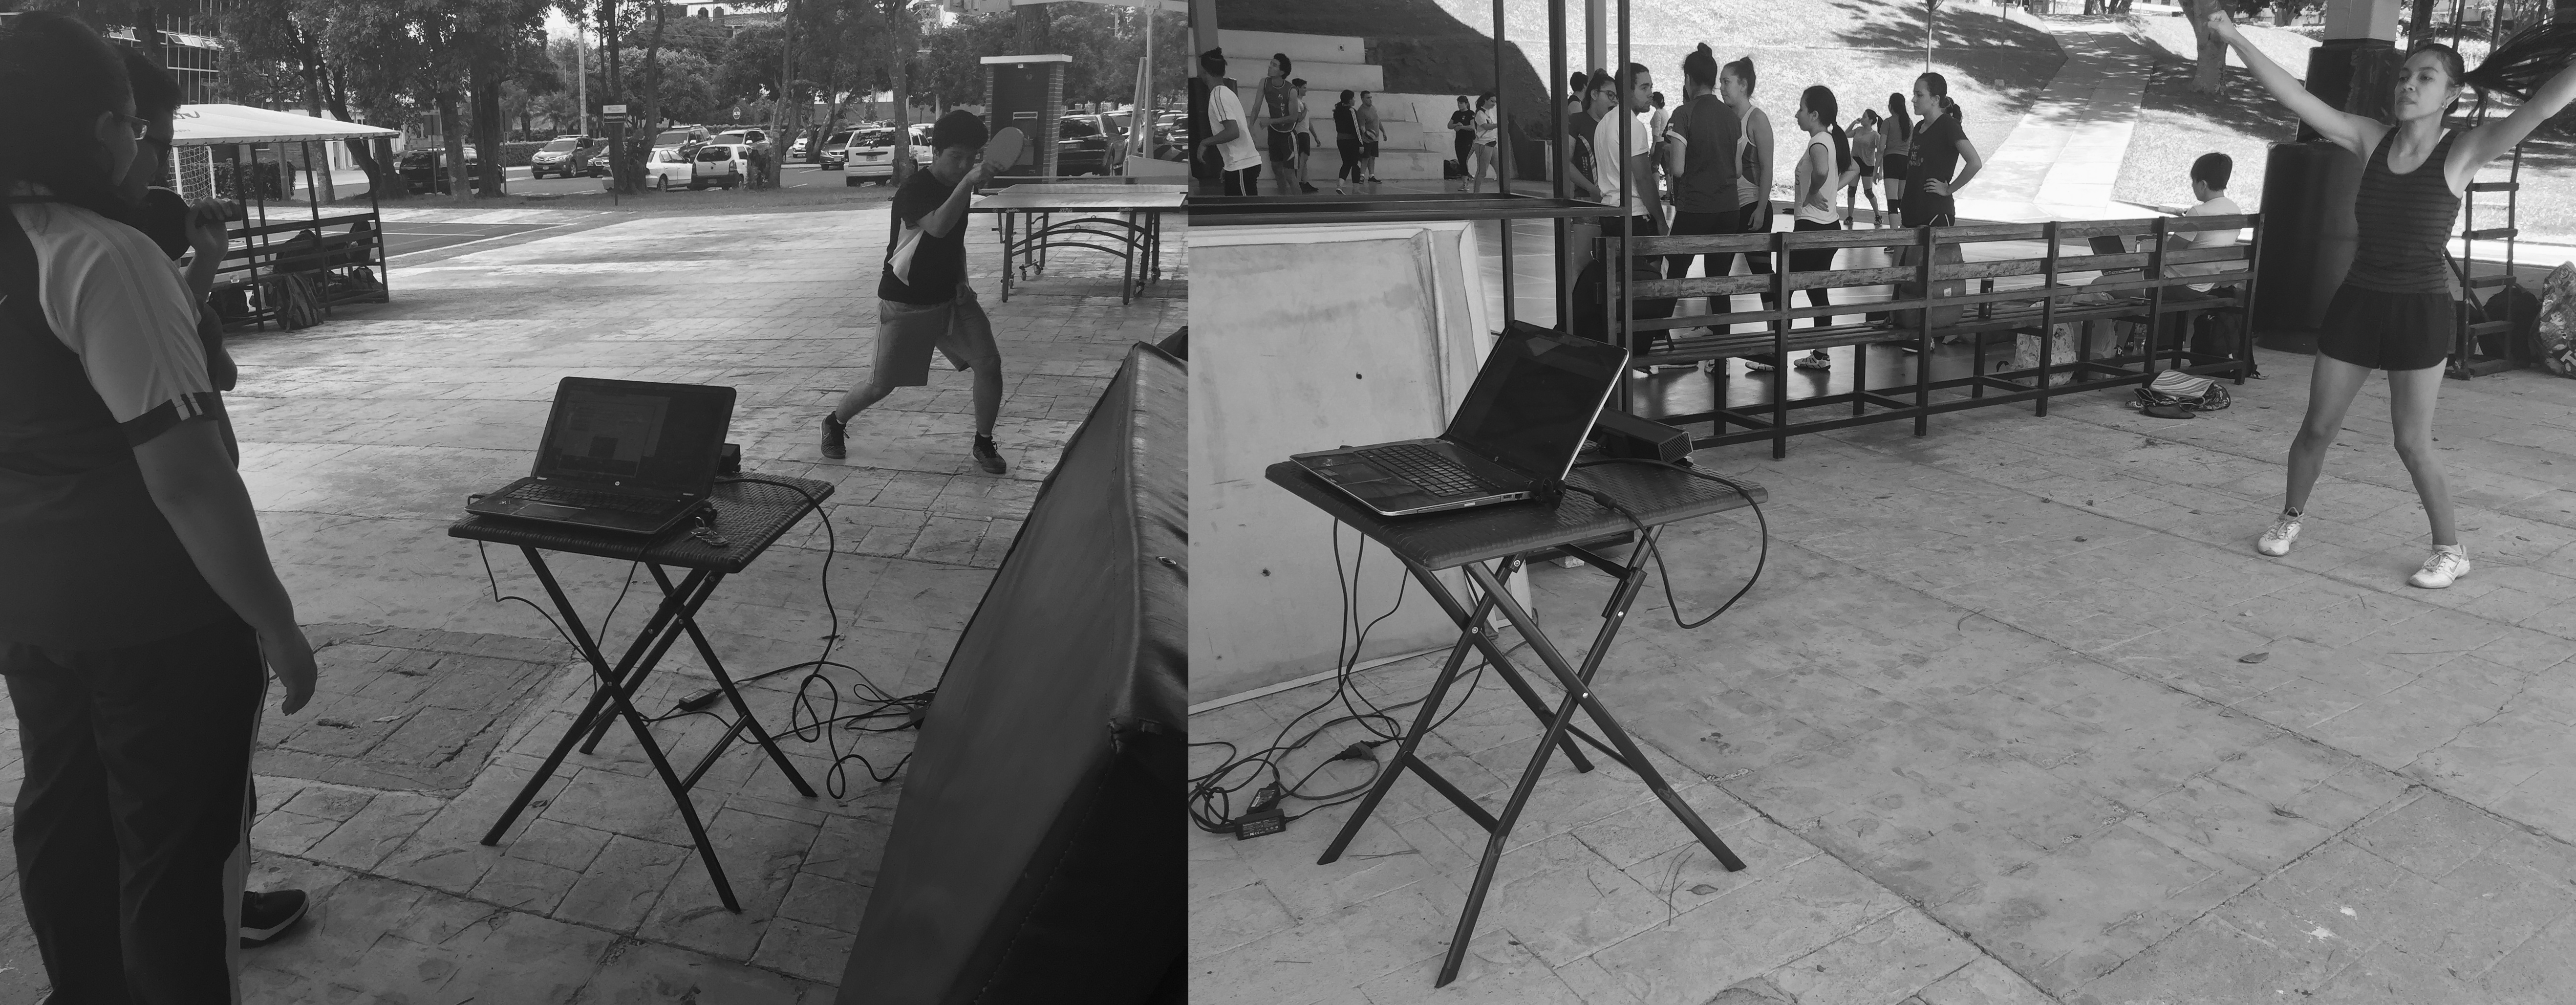
\includegraphics[width=165px,height=165px]{graphics/tabataResultados.png} \\
	\textbf{Fuente:} Propia
\end{figure} 